\documentclass[9pt,twocolumn,twoside]{styles/osajnl}
\usepackage{fancyvrb}
\usepackage[colorinlistoftodos,prependcaption,textsize=normal]{todonotes}
\newcommand{\TODO}[2][]{\todo[color=red!10,inline,#1]{#2}}
\newcommand{\GE}{\TODO{Grammar}}
\newcommand{\SE}{\TODO{Spelling}}
\newcommand{\TE}{\TODO{Term}}
\newcommand{\CE}{\TODO{Citation}}
\journal{i524} 

\title{An overview of Flume and its Applications in BigData }

\author[1,*]{Sahiti Korrapati}

\affil[1]{School of Informatics and Computing, Bloomington, IN 47408, U.S.A.}

\affil[*]{Corresponding authors: sakorrap@iu.edu, S17-IR-2013}

\dates{techpaper-1, \today}

\ociscodes{Flume, Apache Software, BigData}

% replace this with your url in github/gitlab
\doi{\url{https://github.com/sakorrap/sp17-i524/tree/master/paper1/S17-IR-2013/report.pdf}}

\begin{abstract}
This paper provides an overview of Apache Flume and its relevance in BigData. Data Analysis is only half the battle when it comes to Big Data; getting the huge volumes of data to Hadoop is the first step in any Big Data project. Apache Flume comes handy in bringing this data to a centralized store such as Hadoop Distributed File Systems. 
\newline
\end{abstract}

\setboolean{displaycopyright}{true}

\begin{document}

\maketitle

\TODO{This review document is provided for you to achieve your
  best. We have listed a number of obvious opportunities for
  improvement. When improving it, please keep this copy untouched and
  instead focus on improving report.tex. The review does not include
  all possible improvement suggestions and if you sea comment you may
  want to check if this comment applies elsewhere in the document.}

\section{Introduction}

Big Data consists of large volume, high speed, and wide variety of data generated from various sources \cite{tutorialspoint}. Hadoop framework allows for the distributed processing of large data sets across clusters of computers using simple programming models \cite{hadoop}. Apache Flume is one way to get this large data into Hadoop Systems.

According to Apache, Flume is a distributed, reliable, and available service for moving large amounts of data soon after the data is produced. The primary use case for Flume is as a logging system that gathers a set of log files on every machine in a cluster and aggregates them to a centralized persistent store such as the Hadoop Distributed File System (HDFS) \cite{user-manual}.

\section{Architecture}

Flume is an application that allows collecting data from origin logs and sends it to a destination like Hadoop systems. This is achieved by defining dataflows consisting of sources, channels and sinks. These are the three primary structures which make up any Flume dataflow. The  unit of data that flows through Flume is called an event, and the JVM process that runs the dataflow is called agent \cite{user-manual}.

\subsection{Data flow}

\begin{figure}[htbp]
\centering
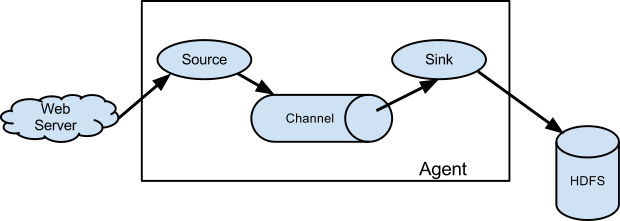
\includegraphics[width=\linewidth]{images/FlumeArchitecture.png}
\caption{Architecture of Flume \cite{user-manual}}
\label{fig:FA}
\end{figure}

Figure \ref{fig:FA} shows the architecture of Flume. An external source delivers events to the Flume source. Flume source receives the event and stores it into its channels. The channel is a pathway between Flume Source and Flume Sink. The sink sends the event to an external repository like HDFS or forwards it to the Flume agent of the next hop in the flow. The source and sink run asynchronously with the events in the channel within the given agent. Events travel through agents of multiple hops before reaching the final destination.
So, Flume allows fan-in and fan-out flows, contextual routing and fail-over routes for failed hops  \cite{cloudera}.

\subsection{Reliability and recover-ability}

The events that are put in channel are removed from it only after they are stored in the channel of next agent or in the terminal repository, maintaining end-to-end reliability of the flow. The transactional approach of the Flume guarantees the reliable delivery of the events.
The end-to-end reliability is guarantied by writing the event to disk in a 'write-ahead log' (WAL). When the agent crashes and restarts, knowledge of the event is not lost. After the event has successfully made its way to the end of its flow, an acknowledgment is sent back to the originating agent so that it knows it no longer needs to store the event on disk. This way, the set of events are reliably passed from point to point in the flow. In case of a multi-hop flow, sink from the previous hop and source from the next hop both run transactions to ensure that the data is safely transferred to the channel of the next hop.

Figure \ref{fig:TI} shows the Transaction Interface of Flume.
\begin{figure}[htbp]
\centering
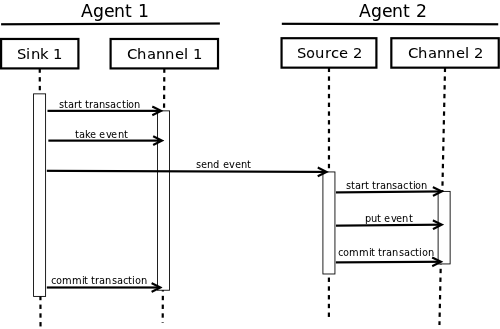
\includegraphics[width=\linewidth]{images/Flume_TI.png}
\caption{Transaction Interface of Flume \cite{dev-manual}}
\label{fig:TI}
\end{figure}

\section{Setup and Configuration}
\subsection{Setting up an agent}
Flume agent configuration is text file in Java properties file format. One or more agents can be configured in the same configuration file which specifies properties of each source, sink and channel in an agent \cite{user-manual}.

\subsection{Starting an Agent}
Shell script called flume-ng in the bin directory of Flume starts an Agent. Agent name, the config directory, and the config file should be specified as arguments as given below \cite{user-manual}:

\begin{quote}
\begin{Verbatim}[numbers=left]
bin/flume-ng agent -n \$agent\_name -c conf 
-f conf/flume-conf.properties.template
\end{Verbatim}
\end{quote}

Properties of Sources, Sinks and Channels should be configured in configuration file. It can be configured as shown below \cite{user-manual}:
\begin{quote}
\begin{Verbatim}[numbers=left]
# Name the components on this agent
a1.sources = r1
a1.sinks = k1
a1.channels = c1

# Describe/configure the source
a1.sources.r1.type = netcat
a1.sources.r1.bind = localhost
a1.sources.r1.port = 41114

# Describe the sink
a1.sinks.k1.type = logger

# Use a channel which buffers events in memory
a1.channels.c1.type = memory
a1.channels.c1.capacity = 1600
a1.channels.c1.transactionCapacity = 100

# Bind the source and sink to the channel
a1.sources.r1.channels = c1
a1.sinks.k1.channel = c1\end{Verbatim}
\end{quote}

Given this configuration file, we can start Flume as follows \cite{user-manual}:
\begin{quote}
\begin{Verbatim}[numbers=left]
bin/flume-ng agent --conf conf 
--conf-file example.conf --name a1 
-Dflume.root.logger=INFO,console
\end{Verbatim}
\end{quote}
Note that in a full deployment we would typically include one more option: --conf=<conf-dir>. The <conf-dir> directory would include a shell script flume-env.sh and potentially a log4j properties file. In this example, we pass a Java option to force Flume to log to the console and we go without a custom environment script \cite{user-manual}.

\subsection{Logging Raw Data}
Flume does not log raw stream of data is not desired in many production environments. Flume attempts to provide clues for debugging the problems like broken pipeline. One way to debug is by connecting an additional Memory Channel connected to a Logger Sink which will output event data to the Flume logs. In some situations, however, this approach is insufficient. For this, Java system properties should be set in addition to log4j properties \cite{user-manual}.

To enable configuration-related logging, set the Java system property $-Dorg.apache.flume.log.printconfig=true$. This can either be passed on the command line or by setting this in the $JAVA\_OPTS$ variable in flume-env.sh.

To enable data logging, set the Java system property -Dorg.apache.flume.log.rawdata=true in the same way described above. For most components, the log4j logging level must also be set to DEBUG or TRACE to make event-specific logging appear in the Flume logs.

Here is an example of enabling both configuration logging and raw data logging while also setting the Log4j loglevel to DEBUG for console output \cite{user-manual}:
\begin{quote}
\begin{Verbatim}[numbers=left]
 bin/flume-ng agent --conf 
 conf --conf-file example.conf 
 --name a1 -Dflume.root.logger=DEBUG,
 console -Dorg.apache.flume.log.printconfig=true 
 -Dorg.apache.flume.log.rawdata=true
\end{Verbatim}
\end{quote}
\section{Experimental Feature}
\subsection{Zoopkeeper based configuration}
Flume supports Agent configurations via Zookeeper. The configuration file is stored in its Node data.  Zookeeper Node tree for agents a1 and a2 will be as follows \cite{user-manual}:
\begin{quote}
\begin{Verbatim}[numbers=left]
- /flume
 |- /a1 [Agent config file]
 |- /a2 [Agent config file]
\end{Verbatim}
\end{quote}

Once the configuration file is uploaded, start the agent with following options \cite{user-manual}
\begin{quote}
\begin{Verbatim}[numbers=left]
bin/flume-ng agent –conf 
conf -z zkhost:2181,zkhost1:2181 
-p /flume –name a1 
-Dflume.root.logger=INFO,console
\end{Verbatim}
\end{quote}

\section{Licensing}
Apache Flume is an open source software licensed under Apache License 2 terms, can be downloaded at Flume website \cite{down}. Source code is available on GitHub \cite{git}.

\section{Use Cases}
Application logs, GPS tracking, social media updates, and digital sensors all constitute fast-moving streams requiring storage in the Hadoop Distributed File System (HDFS). An example of the same is logging twitter data using Flume. Flume helps in gathering data from Twitter API source and storing it in HDFS systems. Flume agent can be configured to catch all the new twitter feeds that appear and automatically transfer them to Hadoop \cite{flume-application}.

\section{Useful Resources}
Flume website has both user manual \cite{user-manual} and developers manual \cite{dev-manual} for further reference which covers how to configure it and use it with examples.
\section{Conclusion}
Some data destined for Hadoop clusters comes from sporadic bulk loading processes, such as database and mainframe offloads and batched data dumps from legacy systems. But what has made data really big in recent years is that most new data is contained in high-throughput streams. Flume efficiently helps in capturing and moving data from these high speed high volume generators to HDFS.

\TODO{well written}

\section*{Acknowledgements}

The authors thank Professor Gregor Von Laszewski and all the AIs of big data class for the guidance and technical support.

% Bibliography

\bibliography{references}
 
\section*{Author Biographies}
\begingroup
\setlength\intextsep{0pt}
\begin{minipage}[t][3.2cm][t]{1.0\columnwidth} % Adjust height [3.2cm] as required for separation of bio photos.
  \noindent
  {\bfseries Sahiti Korrapati} is pursuing her MSc in Data Science from
  Indiana University Bloomington
\end{minipage}
\endgroup
\end{document}
